\documentclass[conference]{IEEEtran}
\IEEEoverridecommandlockouts
% The preceding line is only needed to identify funding in the first footnote. If that is unneeded, please comment it out.
\usepackage{cite}
\usepackage{amsmath,amssymb,amsfonts}
\usepackage{algorithmic}
\usepackage{graphicx}
\usepackage{textcomp}
\usepackage{xcolor}
\usepackage{kotex}
\usepackage{makecell}
\usepackage{float}
\usepackage{subcaption}
\usepackage{tabularx}
\usepackage{longtable}
\usepackage{multicol}
\usepackage{listings}
\usepackage{cleveref, array, booktabs, threeparttable}
\usepackage{array}
\usepackage{tabu} 
\usepackage{enumitem}
\usepackage[export]{adjustbox}
\def\BibTeX{{\rm B\kern-.05em{\sc i\kern-.025em b}\kern-.08em
    T\kern-.1667em\lower.7ex\hbox{E}\kern-.125emX}}
\begin{document}

\title{Soriham\\
{\footnotesize \textsuperscript - Leave Messages via Speaker - }
\thanks
}

\author{\IEEEauthorblockN{Jungi Kim}
\IEEEauthorblockA{\textit{Dept. of Information System} \\
\textit{Hanyang University}\\
Seoul, Republic of Korea\\
damnum3@hanyang.ac.kr}
\and
\IEEEauthorblockN{Raone Park}
\IEEEauthorblockA{\textit{Dept. of Information System} \\
\textit{Hanyang University}\\
Seoul, Republic of Korea\\
raonepark@hanyang.ac.kr}
\and
\IEEEauthorblockN{Yunseok Oh}
\IEEEauthorblockA{\textit{Dept. of Information System} \\
\textit{Hanyang University}\\
Seoul, Republic of Korea\\
grade854@hanyang.ac.kr}\\
}
\maketitle

\begin{abstract}
In the past, we left a note letter on top of the table and used something like post-it to leave messages to other people but as the devices are used often, people started to send messages to a phone. But the problem is that there are so many notifications on the phone that makes people hardly remember the messages they received. Nowadays, more and more devices that are embedded with an AI speaker are being released. So we thought what will it be if we could leave a message on the AI speaker. Soriham is a service that allows a user to leave a message to an AI speaker and reads a received message when the user wants to hear it. Users can leave a message by leaving a voice to an AI Speaker or use an application to write a text message and send it to the AI Speaker. And the AI speaker that received a message will read it when the user wants to read it. Soriham also uses an AI voice mimic system, by gathering users' voice data. By mimicking the voice of the people that the user wants, it will make the users feel friendlier.
\end{abstract}

\begin{IEEEkeywords}
voice, ai speaker, children, message, communication
\end{IEEEkeywords}

\section{Introduction}

\begin{table}[h]
\caption{Role Assignments}
\def\arraystretch{1.24} \small
\begin{tabular}{|p{1.8cm}|p{1.4cm}|p{4.4cm}|}
\hline
Roles & Name & Task description and etc. \\ \hline
User/\par Customer&  Yunseok Oh & Even though developers and managers make a good application, if there is no feedback, it is hard to find unknown errors. He will think of ideas and specify people`s needs, and design functions and application UI. After testing the results of the development team, he will give and feedback from the consumer's point of view. \\ \hline

Software \par Developer & Jungi Kim & oftware developer engages in identifying, designing, installing and testing a software system he has built.  Write codes and make sure it executes. If an error occurs, the developer modifies the code and restart the program and check the services run well. Software developer helps in maintaining and updating the program to ensure that all problems are fixed. The software developer also creates an application that allows users to do specific tasks on an application. \\ \hline

Development \par manager & Raone Park & The development Manager always checks whether each member is performing appropriate tasks and performs the general task of managing the development to proceed success-fully. Developer Manager analyzes what platform will be appropriate to use and find the best one. If there is a problem on the platform, he will try to find the solutions. \\ \hline
\end{tabular}
\end{table}

\subsection{Motivation}
Modern people live a very busy life these days. People are very busy taking care of their careers, hobbies, health, etc. To organize this busy daily life, people usually manage their schedules, write diaries, or simply write notes on their smartphones. However, even if we organize them like that, there are things we forget in our daily lives. Things such as taking out laundry in the washing machine or feeding pets are often forgotten after being immersed in other things. 

It may be simple to prevent forgetting as above. If we hear again about what we have to do or what we have to recognize, we will never forget. Setting an alarm can be a way not to forget, but we thought it would be better to hear what we should do with a familiar voice than to listen to a loud ringtone (or bell sound).

There are also other people who need the voice messages like a young child who don't have smartphones, old people who can't read text well, and disabled people who are uncomfortable communicating through text messages from digital devices. Voice calls are also a good means of communication, but children may not have a smartphone, and adults may not be able to communicate properly at the time they want because they do not always carry it around. And it is hard to call when we are working.

Whether we have to leave a message or listen to the message, there are situations in which we cannot do such things at the exact time we want.
In this case, if we leave a voice message on the speaker in advance, it will be less burdensome for both people who leave a message and who receive the messages. For example, before parents go their work, they can leave a message to their child to take a shower and do homework after school, or someone may leave a message he/she hasn't told the disabled at home before going out.

Voice is an important thing for humans. The voice is the very emblem of the speaker, indelibly woven into the fabric of speech. In this sense, each of our utterances of spoken language carries not only its own message but also, through accent, tone of voice and habitual voice quality it is at the same time an audible declaration of our membership of particular social regional groups, of our individual physical and psychological identity, and of our momentary mood. Voices are also one of the media through which we (successfully, most of the time) recognize other humans who are important to us—members of our family, media personalities, our friends, and enemies. Currently, most of the AI speaker has a limited voice. And the voices that are given may not be satisfied, so if we could mimic the voice of the users we will be able to recognize who is the sender of the message, and feel much friendlier.

\subsection{Research on Related Software}
There are some concepts that uses AI speaker to send a message, mimics a voice by using AI, and reads a schedule that are previously registered.\\

\begin{enumerate}
    \item Kakao\\
    Kakao has released an artificial intelligence speaker called Mini Hexa. Using this speaker, there is a function of checking and sending messages using a pre-registered KakaoTalk account.\\
    \item Google Calender\\
    Google Calendar is a time-management and scheduling calendar service developed by Google. Google Calendar allows users to create and edit events. Reminders can be enabled for events, with options available for type and time. It can also be connected to an AI speaker and ask the schedule that the user registered in advance.\\
    \item Lion Rocket\\
    This company uses deep learning technology to output desired sentences with the voice of the person who wants to enter text. Examples of such voices include one's own voice generation and the voices of famous people such as existing celebrities and presidents. In addition, by developing these technologies, it has the technology to perfectly reproduce the way virtual characters actually speak their voices (like mouth shapes).\\
    \item TypeCast\\
    The company also uses voice AI technology, which has a simpler UI and makes it easy for anyone to extract the desired voice with only text. In addition, there is a great advantage here in that even after setting the voice, the tone of the voice can be adjusted to create a more colorful feeling in the same voice. In addition, the voice created in this way can be downloaded and used as a file.\\
\end{enumerate}

\section{Requirements}
\subsection{Voice Message}
\begin{enumerate}
    \item Leave Messages via voice\\
    Through AI Speaker, users can freely leave messages they want to leave. First, a user wakes up the speaker by calling the speaker's name. After that, the speaker can enter the stage of receiving messages with the user's command "I want to leave a message." The speaker asks the user, "Who is the person who leaves a message?". After the user answers who he/she is (eg. mother, husband), the speaker says, "I checked. Please tell me what message you want to leave" and then receives the user's message. After receiving all the messages, the speaker asks the user once more, "Do you have more messages to add?" and when the user answers "No," it ends, but when the answer is "Yes," it says "Okay. Tell me the message you want to leave" and then receives the user's message.\\
    \item Leave messages via text(application)\\
    If there is a message that the user has failed to leave as a voice on the speaker, he/she can leave a message as text on an external application. After logging in to this application with a social account, the user can leave a message on the connected speaker when the user's account is confirmed that his account is connected to the speaker. The user can leave a message in text in the 'Leave a message' menu in the application. Messages written in text on the application are sent to the speaker and left.\\
    \item Check the messages left\\
    After the user calls and wakes up the speaker, it checks first if there is a message left by someone else with the command "Is there any message left behind?". If there is no message left, the speaker will sleep with a notification saying, "There is no message left behind," and if there is a message left, the speaker will ask, "Do you want to check the message left behind?" When the user answers, "Please check the message left behind," the AI speaker reads the message left behind. If there are multiple messages left, once one message ends, the speaker once again asks the user, "Would you like to check the next message?"\\
\end{enumerate}

\subsection{AI Voice}
\begin{enumerate}
    \item Setting the voice of the speaker similar to user's voice\\
    As above, when the user leaves a message, the speaker asked the user 'who leaves the message'. After dividing the voice by each user, each user's voice is learned so that the speaker's voice can be finally set as the user's voice (or as similar as possible), not the existing AI voice.\\
\end{enumerate}

\subsection{Application}
\begin{enumerate}
    \item Log-in\\
    After downloading an application it will lead to a page that shows us a log-in page. It will ask the user to write down an email address and a password that is previously registered. If the user doesn't have an account, clicking the register button will lead the user to a sign-up page. And if the user has forgotten the password or an id, pressing the find id/password button, will lead the user to the recovery page.\\
    \item Sign-up\\
    On the sign-up page, the user should enter a name, gender, and choose a voice that a user wants to use. If the user wants to add a new voice, the user should check the permission from the application to gather voice data.\\
    \item Leave a Text Message\\
    To leave a message to an AI speaker, users should choose what speaker they want to send, write down a message and press send button. If the user wants to reserve a text message to send it at a specific time, press the reserve button and choose the specific time that the user wants.\\
    \item Manage sent messages\\
    To delete the sent message, users should press a text message long time to see a small menu and choose the delete button. And if the users want to change a sent message to a reserve message, press a text message long time and choose the reserve button from a small menu, and choose the change to reserve button.\\
\end{enumerate}

\section{Development Environment}

\subsection{Choice of Software Development Platform}
\begin{enumerate}
    \item Platform
    \begin{itemize}
        \item Android\\
        “Soriham” needs to be on a mobile platform for quick access and easy use. So, for our program, we have chosen the Android mobile operating system as the platform. Android is the best-selling mobile OS in the world, which has the largest mobile OS share which is about 71\%. And also, software for development on Android is widely available and it`s free.\\
    \end{itemize}
    \item Programming Language
    \begin{enumerate}
        \item JavaScript\\
        JavaScript is an object-based script language mainly used in web browsers along with HTML and CSS. HTML gives meaning to raw content, CSS formats the displayed content, and finally JavaScript interactive content and formatting.
        It is an advanced multi-paradigm and supports event-based, functional, and command-type programming styles. Despite the original purpose of creating a web browser, it is now possible to build a server. JavaScript is also platform-independent. This is the main reason why we choose JavaScript. In particular, React-native is used as the front end and Node.js is used as the backend.\\
        \item Python\\
        Python is interpreted, object-oriented, and high level. The programming language Python supports modules and packages. Its interpreter and extensive standard library are available in source or binary form free of charge for all major platforms and are freely distributed.\\
    \end{enumerate}
    \item Development Environment
    \begin{enumerate}
        \item React-Native\\
        React Native is an open-source mobile application framework developed by Facebook. It is used to develop applications for Android, iOS, Web, and UWP, and allows developers to use React along with native platform functions.\\
        \item TensorFlow\\
        TensorFlow is an open-source library that is popular with Machine Learning. TensorFlow offers APIs that facilitate Machine Learning. The goal is to implement this AI model in using NUGU speakers.\\
        \item NUGU Playbuilder\\
        NUGU Playbuilder connects to NUGU speaker to support SK Telecom's artificial intelligence speaker NUGU various services. Whose platform first identifies the user's intention to speak through speech recognition and natural language understanding. Then, it behaves and reacts appropriately in text-to-speech. NUGU Playbuilder is a GUI-based integrated development environment that provides the necessary technology for this process.\\
        \item Amazon EC2\\
        Amazon Elastic Compute Cloud (EC2) forms the center of Amazon's cloud computing platform Amazon Web Services, allowing users to rent virtual computers and run their own computer applications on them. We use this for backend development.\\
        \item MySQL\\
        SQL is a stable and consistent database form. Among them, MySQL is the most widely used open-source relational SQL database management system. MySQL is one of the best RDBMS used to develop various web-based software applications. We chose SQL instead of NoSQL because of the nature of the database.\\
        \item Git and Github\\
        Git and Github offer three main functions. The first is version control. Git is a version control system that stores the timing and content of changes to the file. The second is backup. If the data is stored only on the local computer, the data will be lost and must be saved. GitHub is Git's remote repository that provides online backup. Finally, Github offers strong collaboration capabilities. When people work as a team, they can push and pull source code to remote storage to work together.\\
        \item Visual Paradigm\\
        It is a UML CASE tool that supports UML2, SysML, and Business Process Modeling Notation (BPMN) of the Object Management Group (OMG). In addition to modeling support, it also provides report generation and code engineering functions, including code generation. It is possible to reverse engineer diagrams in code and provide reciprocating engineering for various programming languages.\\
    \end{enumerate}
\end{enumerate}

\subsection{Software in use}
There are companies that use AI speaker to send messages to a phone such as "Mini Hexa" which is from Kakao, "Giga Genie" from KT, and "Google Home" from Google. However, our "Soriham" differs from existing services in that it has the function of reading the messages that are sent from a phone. 

And there are some companies that use AI voice to read a text message such as "Lion Rocket" and "TypeCast". However, "Soriham" uses not only an AI voice that is previously registered, but it also gathers data of a voice of a user and speaks with the user's voice when enough data is stored.\\

\subsection{Task Distribution}

\begin{table}[htbp]
\begin{center}
\caption{Task Distribution}
\begin{tabular}{|l|l|}
\hline
Name        & Task description          \\ \hline
Yunseok Oh  & Backend                   \\ \hline
Jungi Kim   & Frontend, Play Builder    \\ \hline
Raone Park  & Frontend, Play Builder    \\ \hline
\end{tabular}
\end{center}
\end{table}
Task Distribution is shown in Table 2. Each member has his own main role, but since we do not know much about programming, we ask each other, share our thoughts and ideas to improve our project, and proceeds.\\

\section{Specifications}

\subsection{AI Speaker}
\begin{enumerate}
    \item Voice Message
    \begin{enumerate}
        \item Leave a message using voice\\
        - The speaker receives the message when the user asks the speaker to receive a voice message.
        
        - When the user asks to start a message mode "소리함 켜줘", the speaker will ask the name of the sender "작성자의 이름이 무엇인가요?" the time that the message will arrive, "언제 메세지를 남겨드릴까요?" the message that user wants to send, "남기실 메세지를 말씀해 주세요" and confirmation message."000님이 몇시에 말씀하신 메세지가 ~ 로 남길까요?"
        
        - If the user says "응 남겨줘", the speaker will send a message but if the user says "틀렸어 다시해줘", "시간 몇시로 바꿔줘", "이름을 000로 바꿔줘", "메세지 바꿔줘" and the speaker will change the specific part that the user asked to do and asked the confirmation message again.\\
        \item Message left using text in app\\
        - In the application, the user could go to the messenger part, write down the messages that the user wants to send, and it will be sent to the speaker.
        
        - The speaker receives the text message that the user sent on the application.\\
        \item Adjust the received messages\\
        - If the Speaker receives a message, the speaker will give a ringtone as a signal.
        
        - If there are unread messages in the speaker, the led of the speaker will blink.
        
        - User could check the messages by asking a speaker to read them.
        
        - Users could check how many messages there are by asking "메세지 몇개 있어?" and the speaker will reply, "현재 몇개의 메세지가 있습니다."
        
        - User could delete the received messages by asking "메세지 삭제해줘". And the speaker will reply "삭제되었습니다".
    \end{enumerate}
    
    \item Voice
    \begin{enumerate}
        \item Basic Voice\\
        - There are several voices that are given, and the users could choose a voice that they want to send a message. Users can choose the voice depending on the mood, emotion, and feelings that the user currently has
        
        - By the voice that the user chose, the speaker will read the message.\\
        \item AI Voice
        \begin{itemize}
        \item Voice machine learning\\
        - By following the steps, the user could record their voice to TTS.
        
        - If the record is successfully done, the voice of the user will be a part of the voice option. 
        
        - If the user chooses a voice to a voice that the user recorded, the user will be able to ask the speaker to read text messages using the user's voice.
        \end{itemize}
    \end{enumerate}
\end{enumerate}

\subsection{Application}
\begin{enumerate}
    \begin{figure}[ht!]
    \centerline{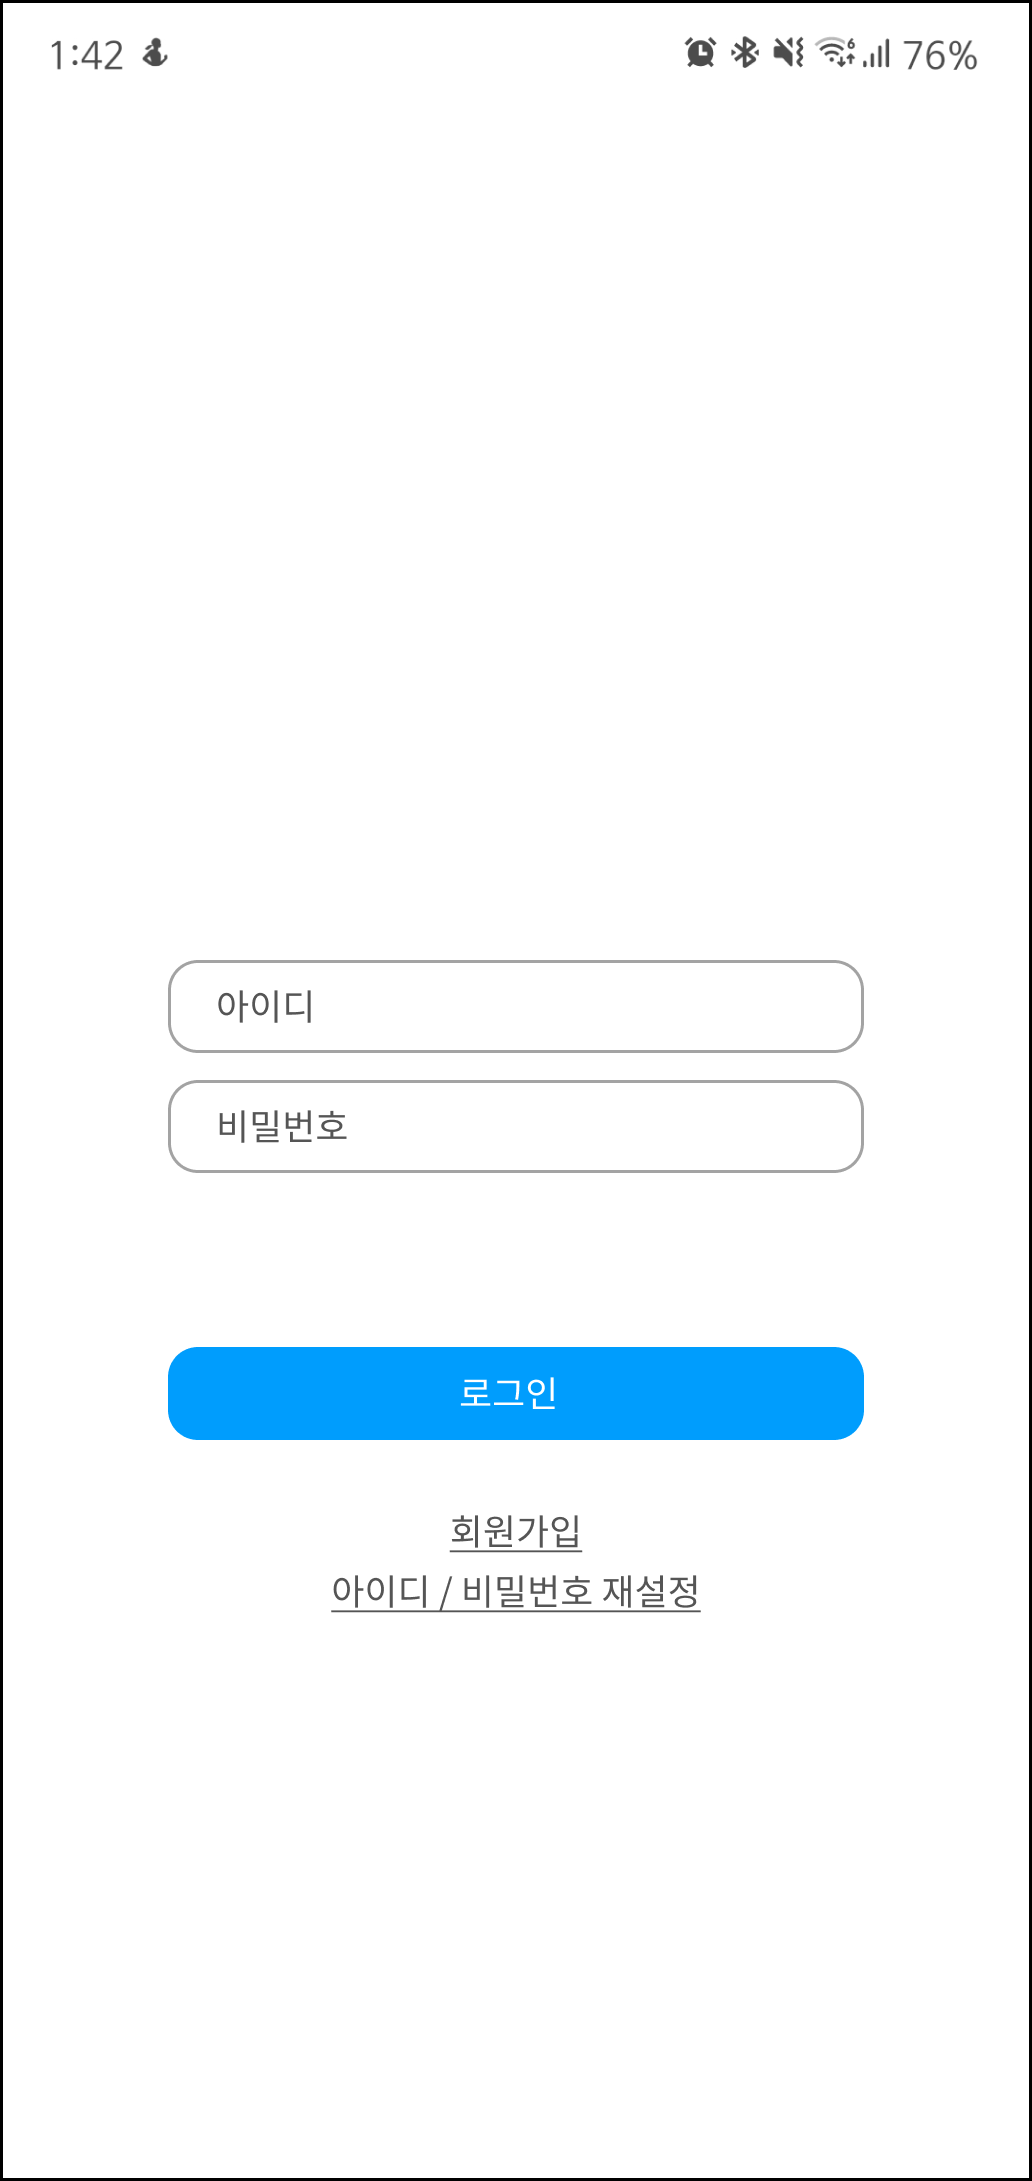
\includegraphics[width=4cm]{img/Login.png}}
    \caption{Login}
    \end{figure}  
    \item Login [Fig.1]\\
    - The user could login through typing a ID that is registered in SKT NUGU Smart Home.
    
    - After the user succeeds in logging in, the user goes to the main page where 'send messages' and 'voice setting' menu are existing.\\
    
    \begin{figure}[ht!]
    \centerline{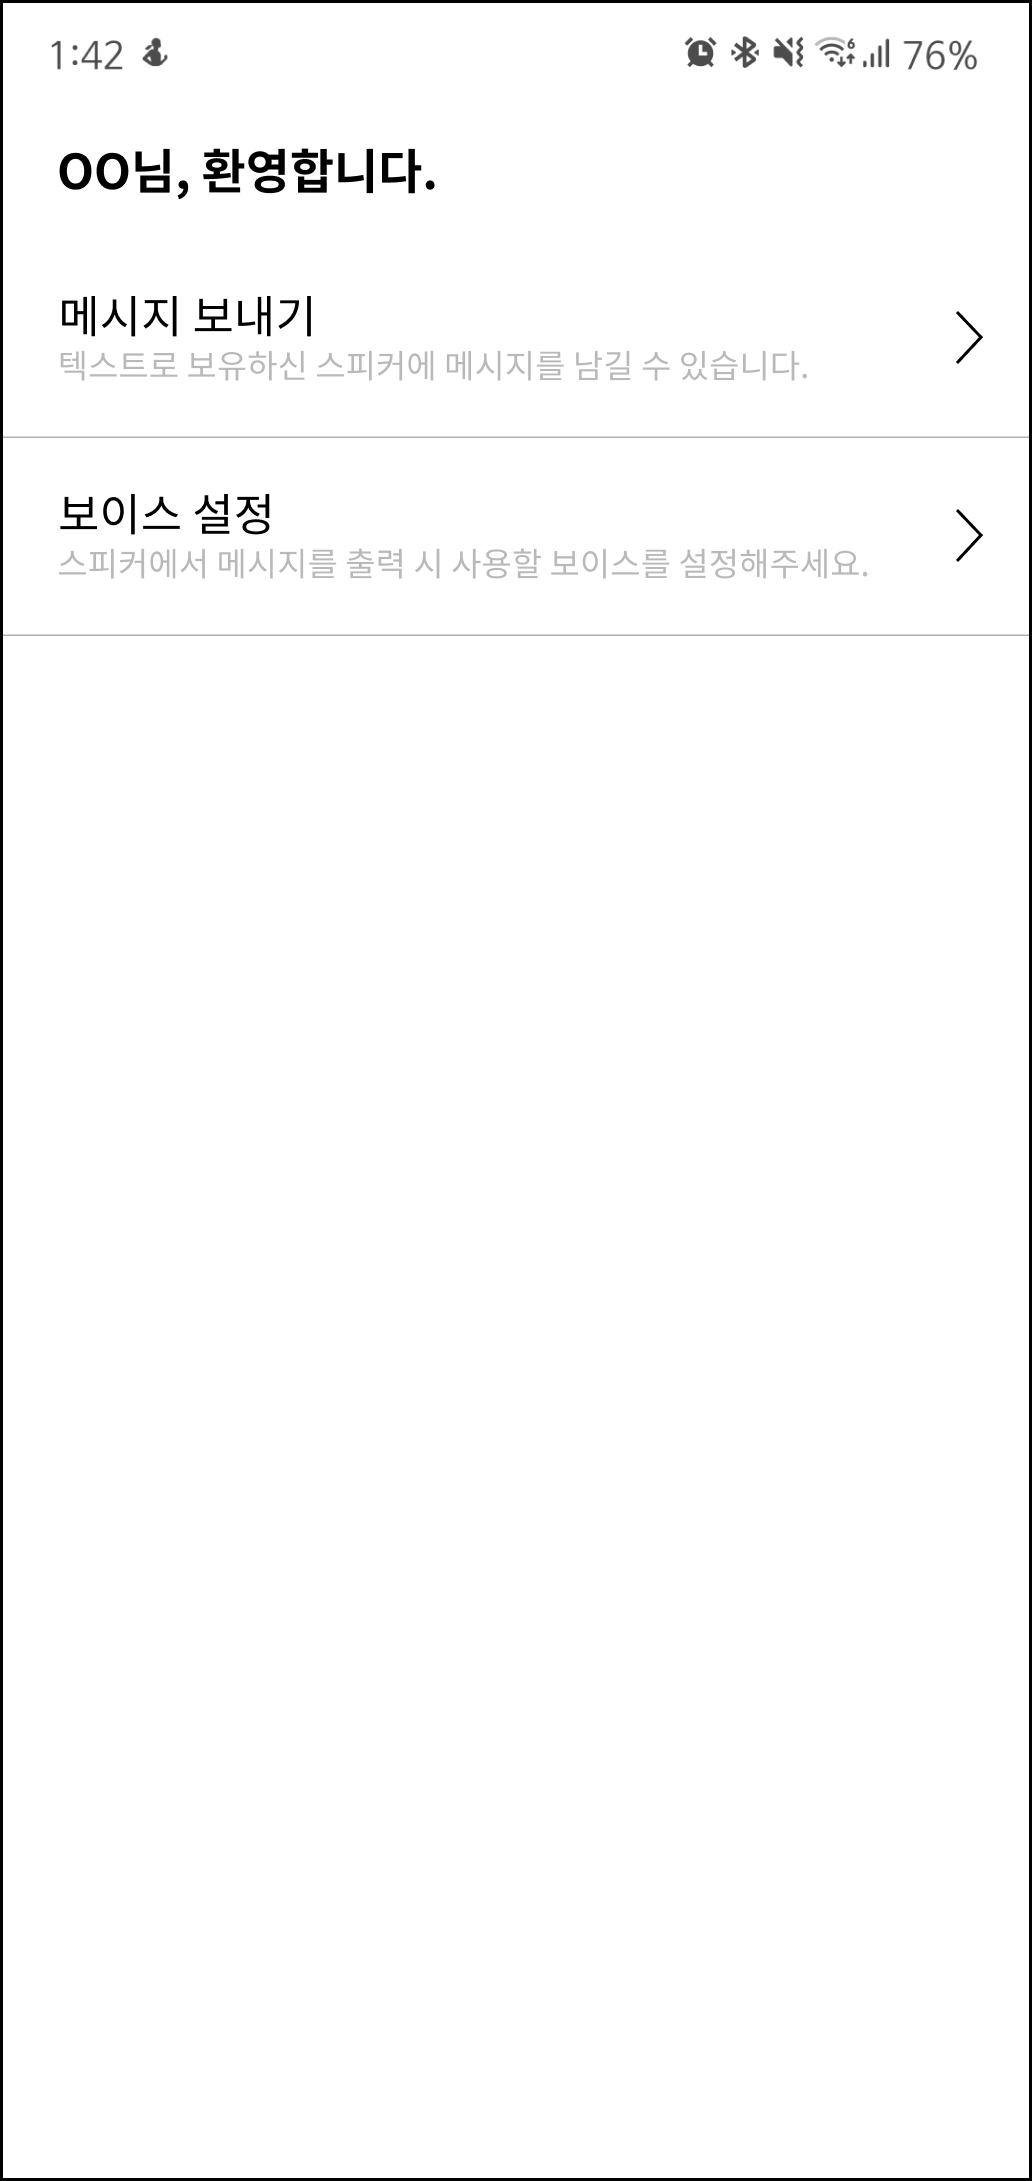
\includegraphics[width=4cm]{img/Main.png}}
    \caption{Main}
    \end{figure}  
    \item Main Page [Fig.2]\\
    - There are two menus, to send a message and a Voice setting that a user wants to send.
    
    - When the user chooses the first option which is to send a message, it will lead the user to Send Message page.
    
    - When the user chooses the option which is voice setting, it will lead the user to the Voice Setting page.\\
    
    \begin{figure}[ht!]
    \centerline{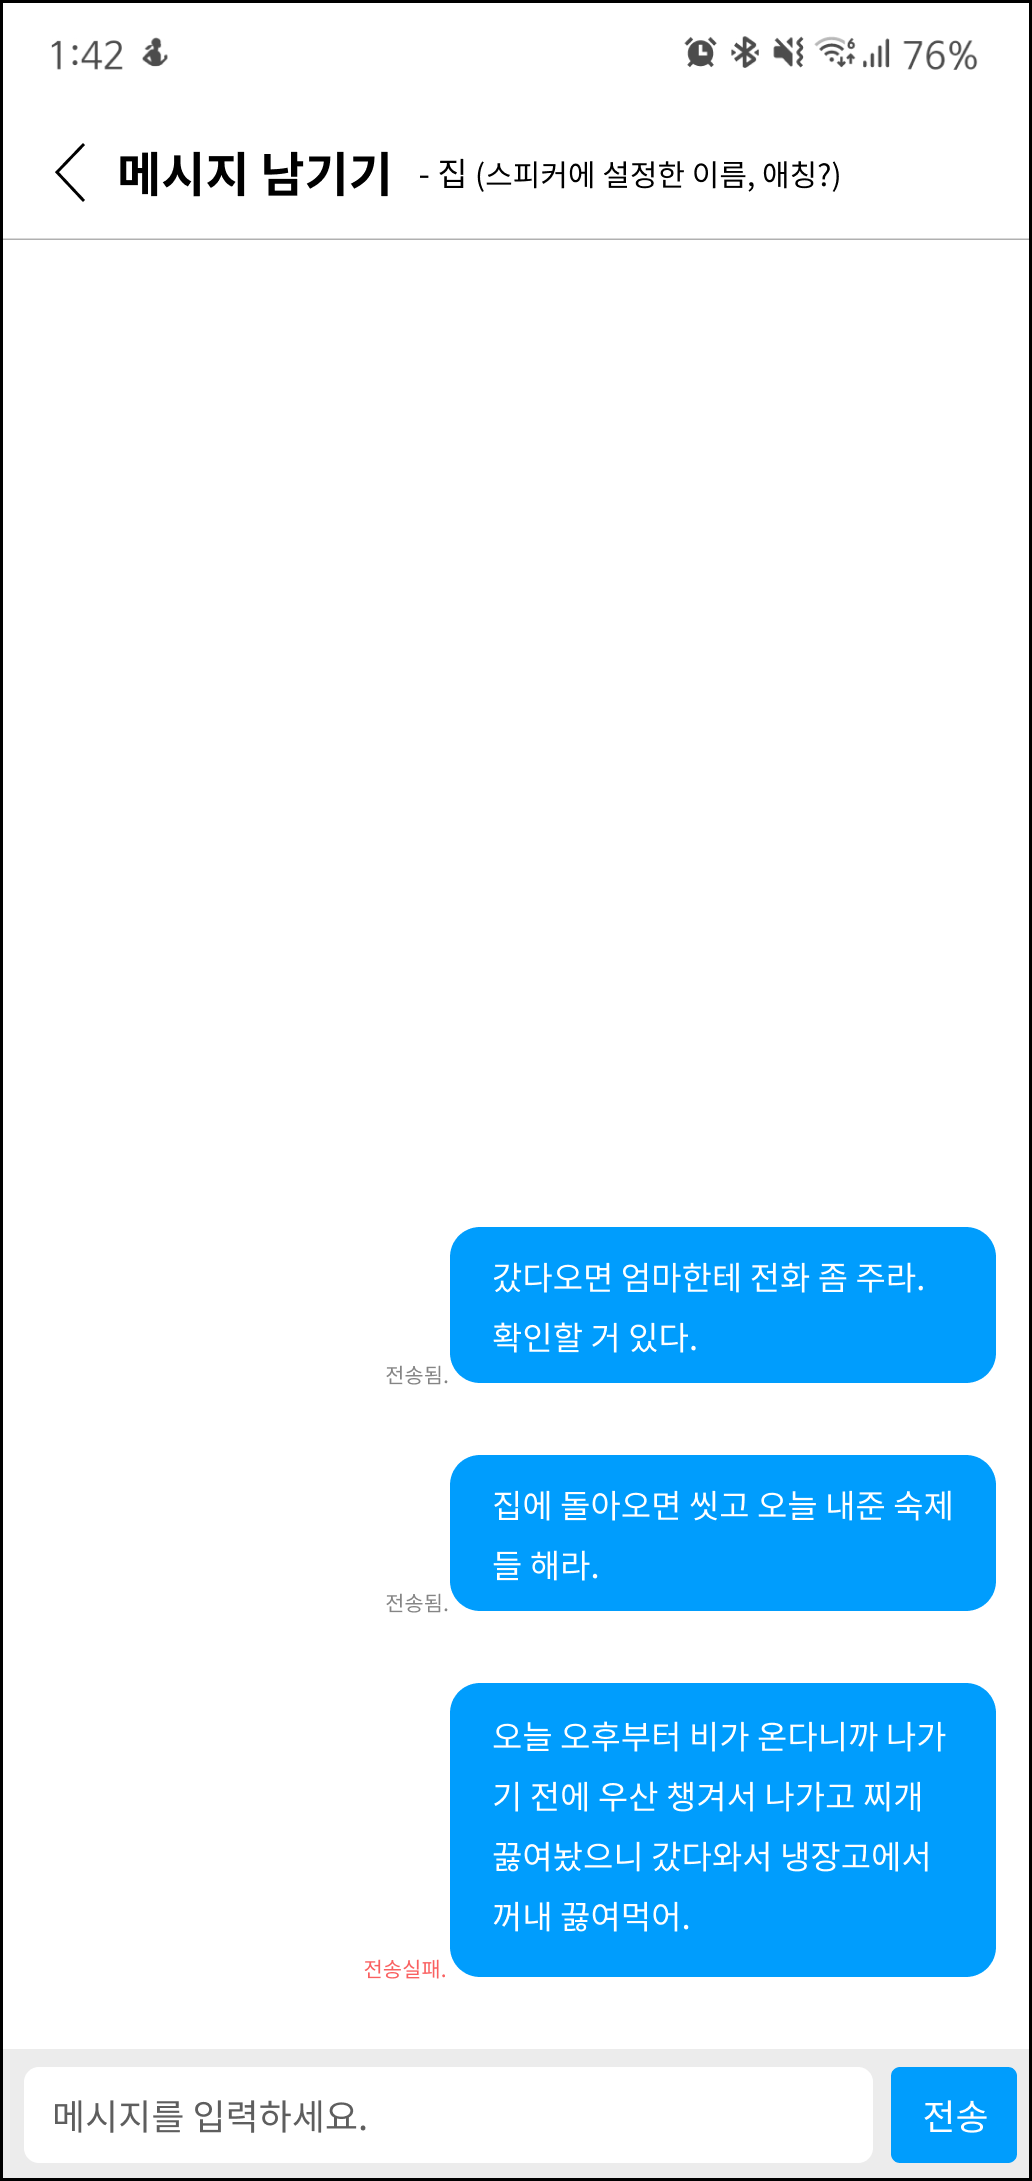
\includegraphics[width=4cm]{img/Message.png}}
    \caption{Send Messages}
    \end{figure}  
    \item Send Message [Fig.3]\\
    - The user could type a message and send it by pressing the send button.
    
    - The length of the message cannot exceed 140 characters in English and 70 characters in Korean.
    
    - If the message entered in text was well sent to the speaker, the mark '전송됨' appears next to the message sent. But if not, '전송실패' appears. The user can resent the failed message using copy and paste.
    
    - By pressing a sent message for 3 seconds, the delete button will pop out.
    
    - If someone else hears a message sent in text through a speaker, the "전송됨" mark will be changed to a "읽음" mark. Messages changed to "읽음" marks cannot be deleted.
    
    - On the top left, there is a button that lets the user go back to the Main page.\\
    
    \begin{figure}[ht!]
    \centerline{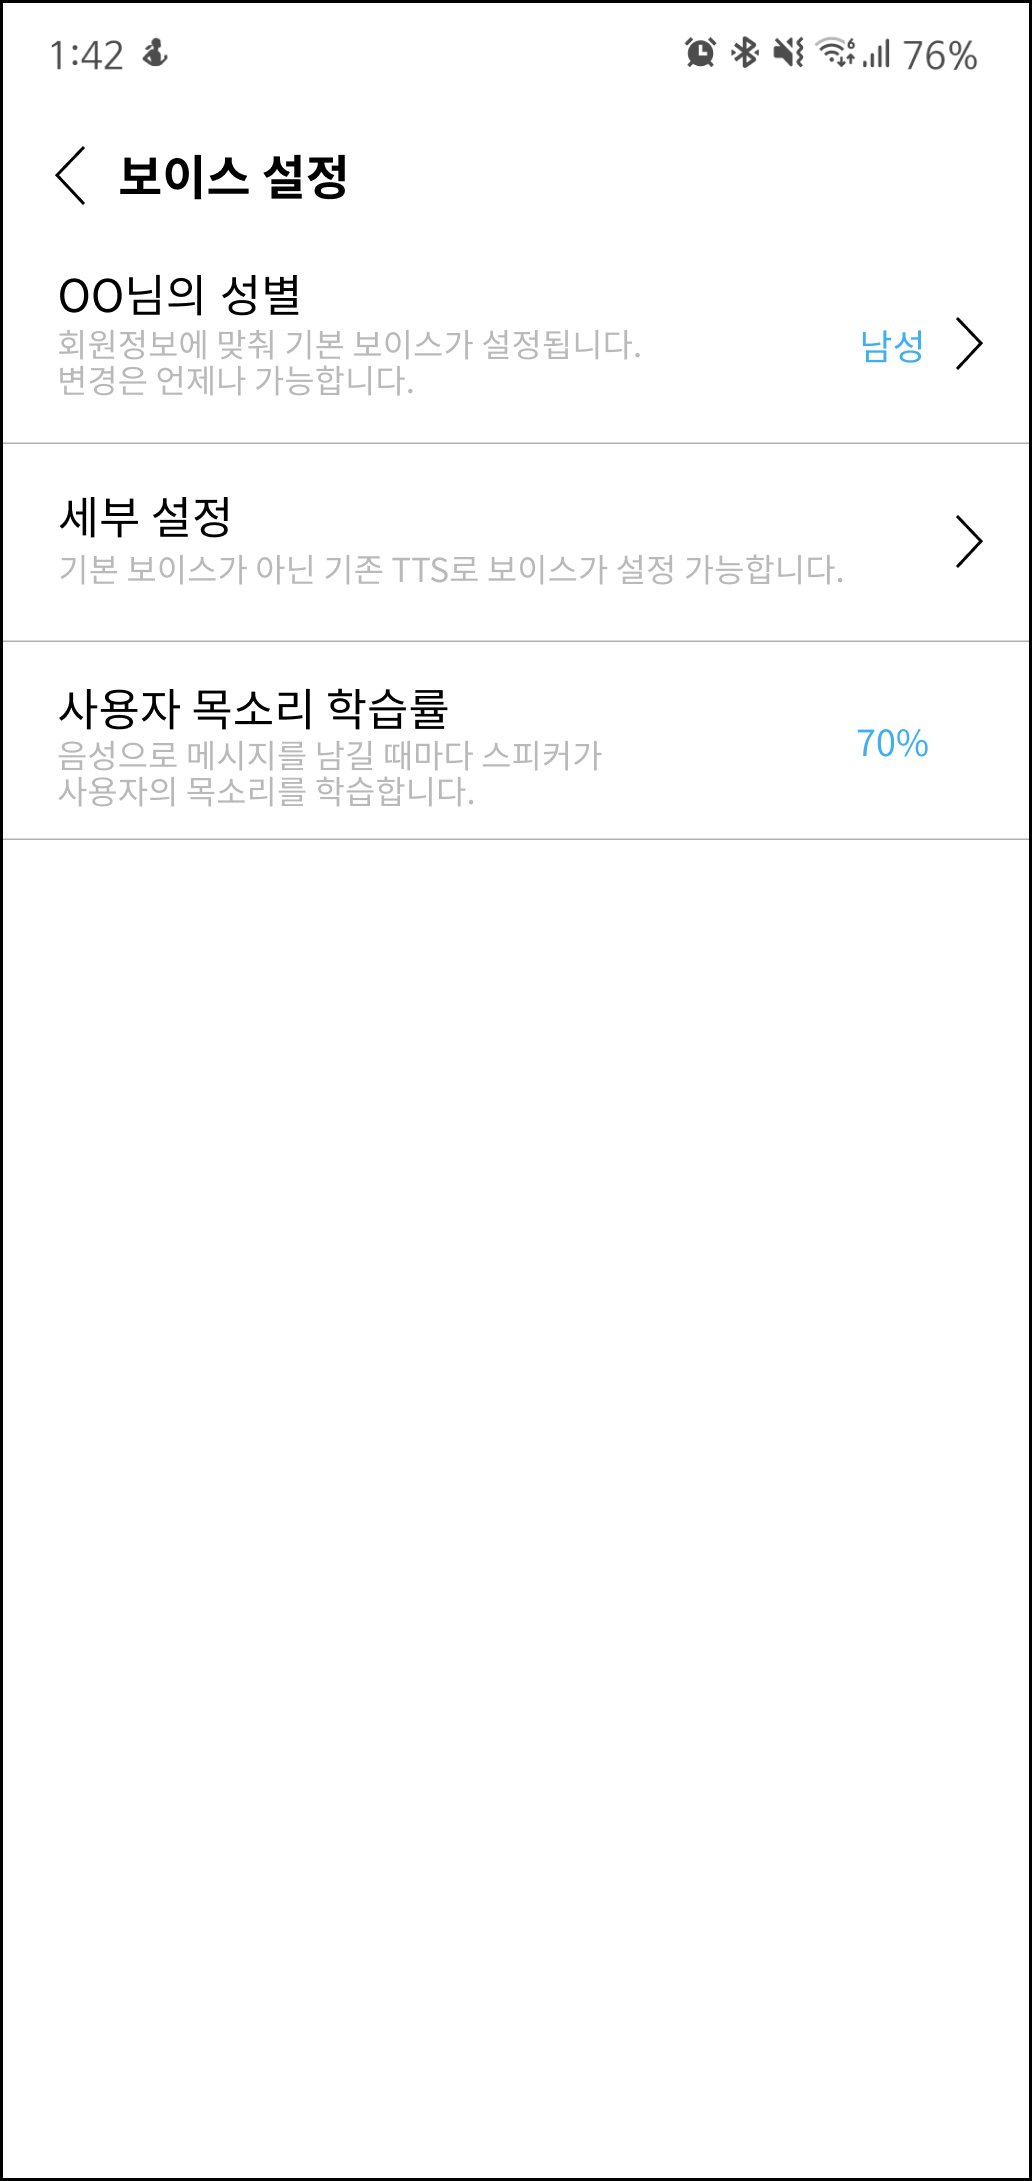
\includegraphics[width=4cm]{img/Setting - Voice.png}}
    \caption{Voice Setting}
    \end{figure} 
    \item Voice Setting [Fig.4]
    \begin{enumerate}
        \item Gender\\
        - The default gender setting follows the information entered when the user registered.
        
        - The user can change between the two (male/female) anytime the user wants.\\
        
        \begin{figure}[ht!]
        \centerline{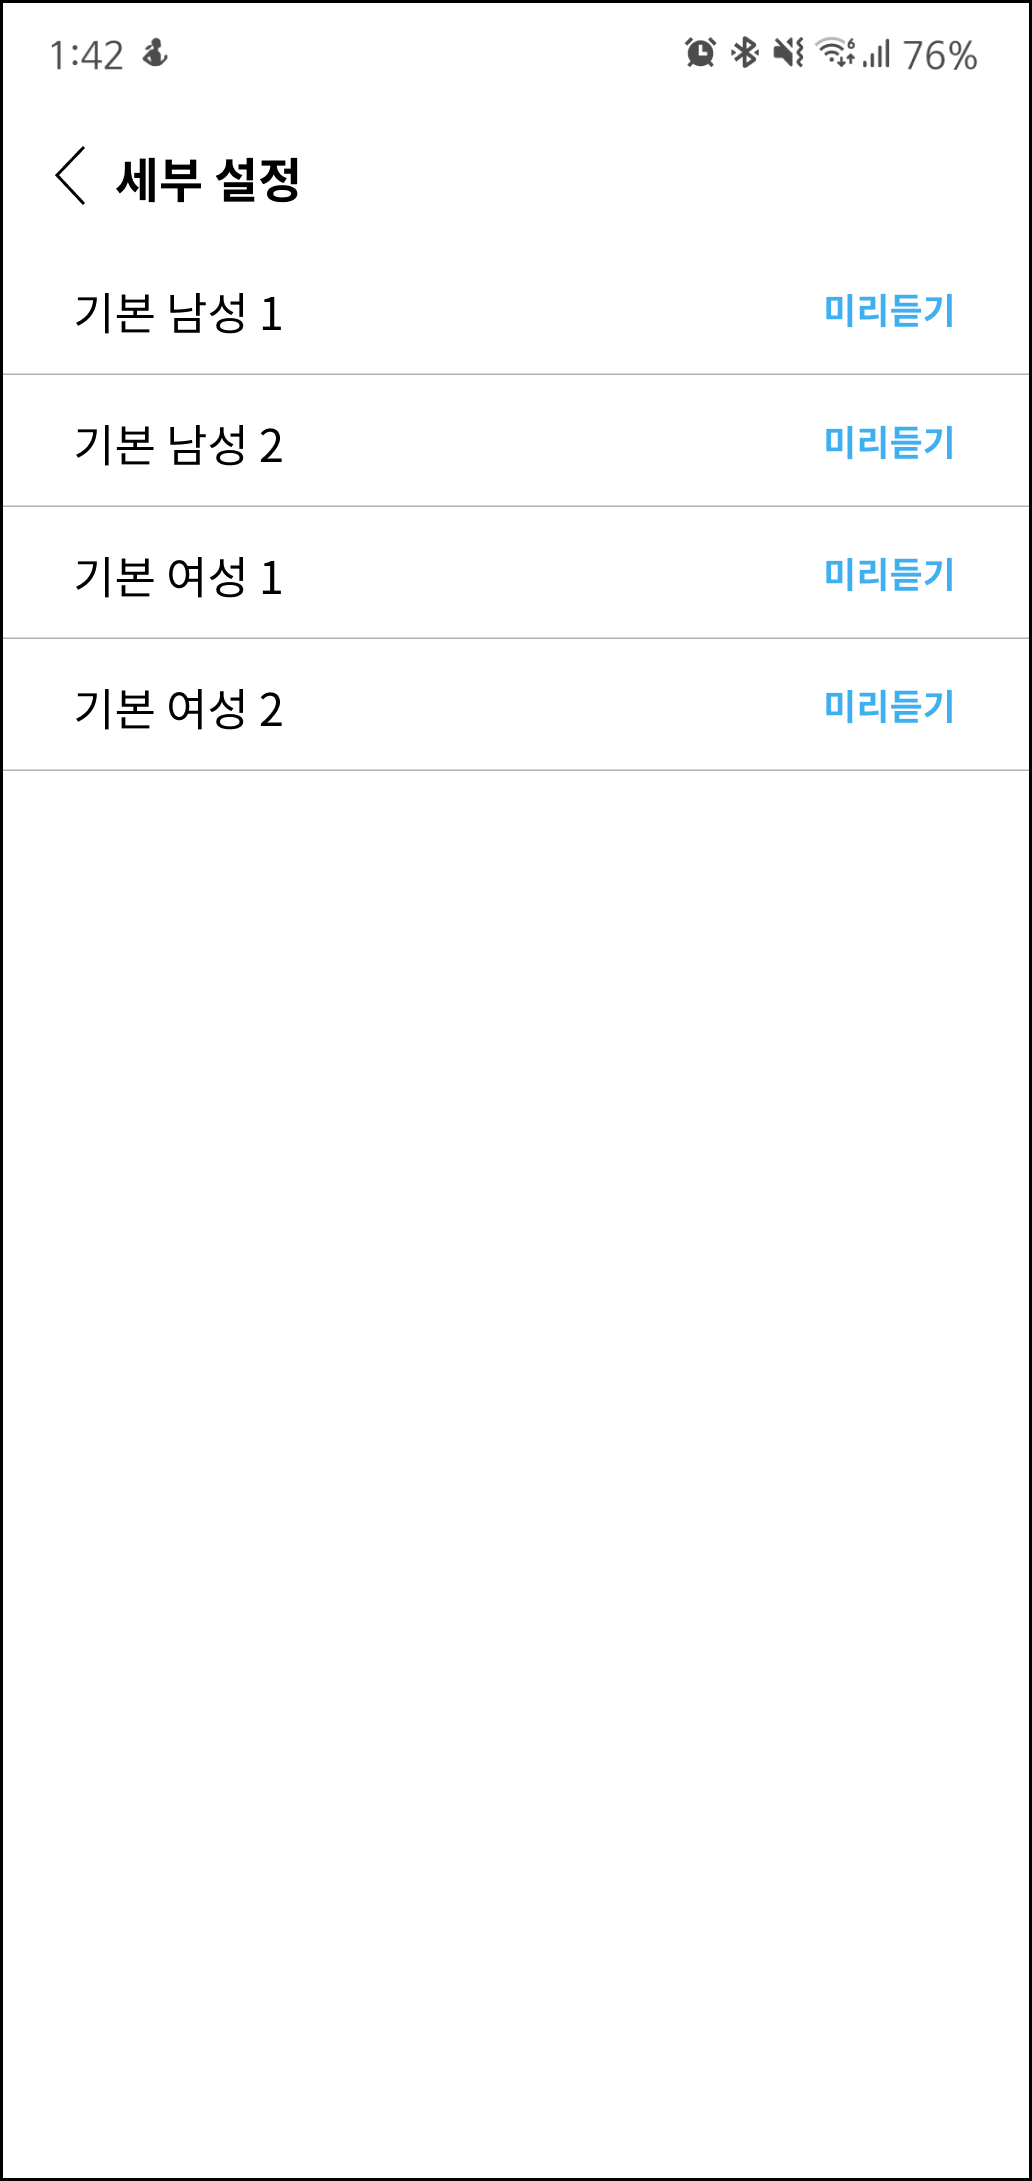
\includegraphics[width=4cm]{img/Setting - Voice - Detail.png}}
        \caption{Voice Detail Setting}
        \end{figure} 
        \item Voice Detail [Fig.5]\\
        - Users can set their voice with the existing TTS, not the user's own voice.
        
        - The user can listen to the sample voice by pressing the '미리듣기' button for each TTS before choosing a voice.
        
        - If enough data is gathered for AI voice, users could choose an option to use AI voice.\\
    \end{enumerate}
\end{enumerate}

\section{Architecture Design \& Implementation}
\subsection{Overall Architecture}
- Soriham is divided into two main modules: the frontend and the backend (see Figure). The frontend is compatible with its own git and is available on Android or IOS devices. Send a request to the backend server to get data when you are connected to the Internet using this application(program).

- The backend server has two endpoints (who, message). The server performs the necessary tasks based on what AI Speaker requests. If a user uses a request to “save”, the backend server identifies who it is with a parameter called who, determines which message it is, and stores it in the database. For example, when a father saves the message "Eat dinner" on a server, “who” is the father, and “message” is "Eat dinner" and then saves it.
In addition, two endpoints (who, message) are also used when using the message import function. When a user requests to retrieve a message, the backend server identifies who came with a parameter called “who”, requests the stored message to the TTS server, converts it into the person's TTS, and responds to the backend server.

- When response from the TTS server arrives on the backend server, the server responds to the data back to the AI Speaker and processes it in a way that is played by the AI Speaker.\\

\subsection{Directory Organization}
- Not Yet\\

\subsection{Modules}
\begin{enumerate}
    \item Module 1. Database\\
    - The database that is used for Soriham is a MySQL-server database and it is connected to the server. In application, all of the messages that are written will be sent to the database. All of the messages will be sent with a tag that a user-selected. If the user selected a certain voice, a message will be tagged according to it. The data that is stored in the database will be sent to the TTS API. According to a tag, different voices will be converted to mp3 files. To let NUGUplayBuilder play the file, it will be converted to an m3u8 file. When the user chooses to use their own voice, the message data will be sent to a Speech to Text Machine Learning module, and it will be converted to a user's voice m3u8 file.  After the files are converted, it will wait for the signal from NUGUplayBuilder. When NUGUplayBuilder asks for the data, the converted data will be sent to NUGUplayBuilder.\\
    \item Module 2. TTS (Text-to-Speech)\\
    - Since a database cannot be directly converted to Speech, TTS API is needed. TTS can turn text into natural-sounding speech in 220+ voices across 40+ languages and variants with an API powered by Google's machine learning technology.\\
    \item Module 3. Machine Learning\\
    - Soriham uses two machine learning learning models: Glow-TTS and HiFiGAN-TTS for voice learning. The user directly records a certain amount of sentence files through the microphone to produce base data. Machine learning is conducted based on the produced recording file. It determines the overall voice tone of the user through Glow-TTS. Use HiFiGan-TTS to create a model that is closer to the user's actual voice. As the time of machine learning increases, it gets closer and closer to the user's actual voice. After the learning is completed, the two learned data are synthesized to extract the learning results of the user's voice based on the data.\\
    \item Module 4. App\\
    - Soriham application is oriented for both Android Ios. We use react-native for our development IDE. There are Login, Menu, Voice Setting, and Send message contents in the application. The application allows users to communicate with the Soriham. It receives a message that the speaker spoke on the speaker when the speaker is in Soriham mode. The message from a speaker will be shown on the application. And when the user sends a message through an application, it will be sent to a speaker and reads when the user asks. The application allows users to choose voices. When the user chooses a certain voice, the text message will be converted to it.\\
    \item Module 5. NUGU Playbuilder\\
    - We use Nugu Play Builder to connect intents from users with actions to run on speakers. There are two types of intents: SoundRecordIntent and SoundPlayIntent. 'SoundRecordIntent' executes 'SoundRecordAction'. SoundRecordIntent has an entity called "VOICE\_TYPE" to decide which voice of people who trained their voice into the machine learning model is used later. "SoundPlayIntent" executes "SoundPlayAction" and has a parameter called "sound\_type," which is consistent with "VOICE\_TYPE" set by "SoundRecordAction." The message will be played with the voice you specified when recording the voice.\\
\end{enumerate}

\section{Use Cases}

\subsection{User Case 1: Leave Messages Using Voice}
\begin{figure}[ht!]
    \centerline{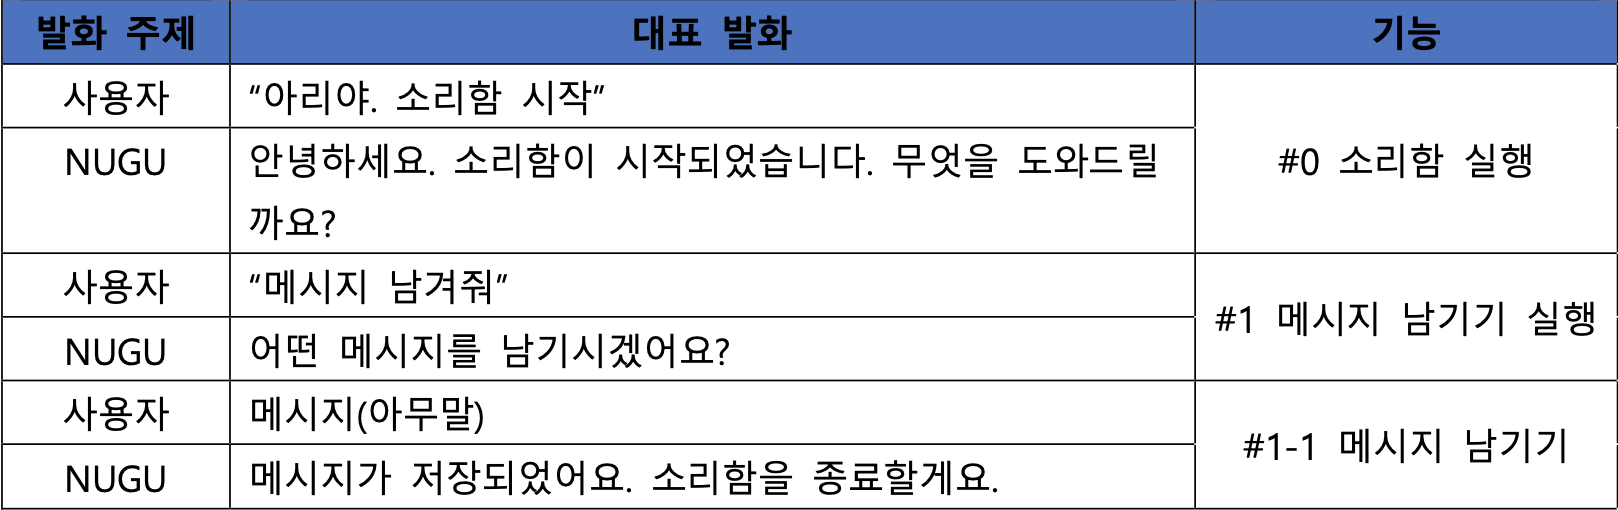
\includegraphics[width=9cm]{img/usecase 1.png}}
    \caption{User Case 1}
\end{figure}
- Users can leave messages using speakers at any time they want. After the user wakes up the speaker first, the user reveals his intention by saying, "I want to leave a message." Then, the speaker grasps the intention and takes 'SoundRecordAction'. When the user leaves a message he or she wants to leave, the voice turns into text(Speech-to-Text) and moves on to the server. The text is changed to the user's voice learned through the learning model and turns into the voice (Text-to-Speech). The voice file is stored in cloud storage.\\

\subsection{User Case 2: Leave Messages Using Text in App}
- Users can also leave messages not only using voice, but also text. If you write down the message you want to leave on the application as text and press the send button, the text will be delivered to the learning model. Text is changed to the user's voice through a learning model and stored as a voice file(it can be 'mp3' or 'm3u8').\\

\subsection{User Case 3: Playing Messages Left Before}
\begin{figure}[ht!]
    \centerline{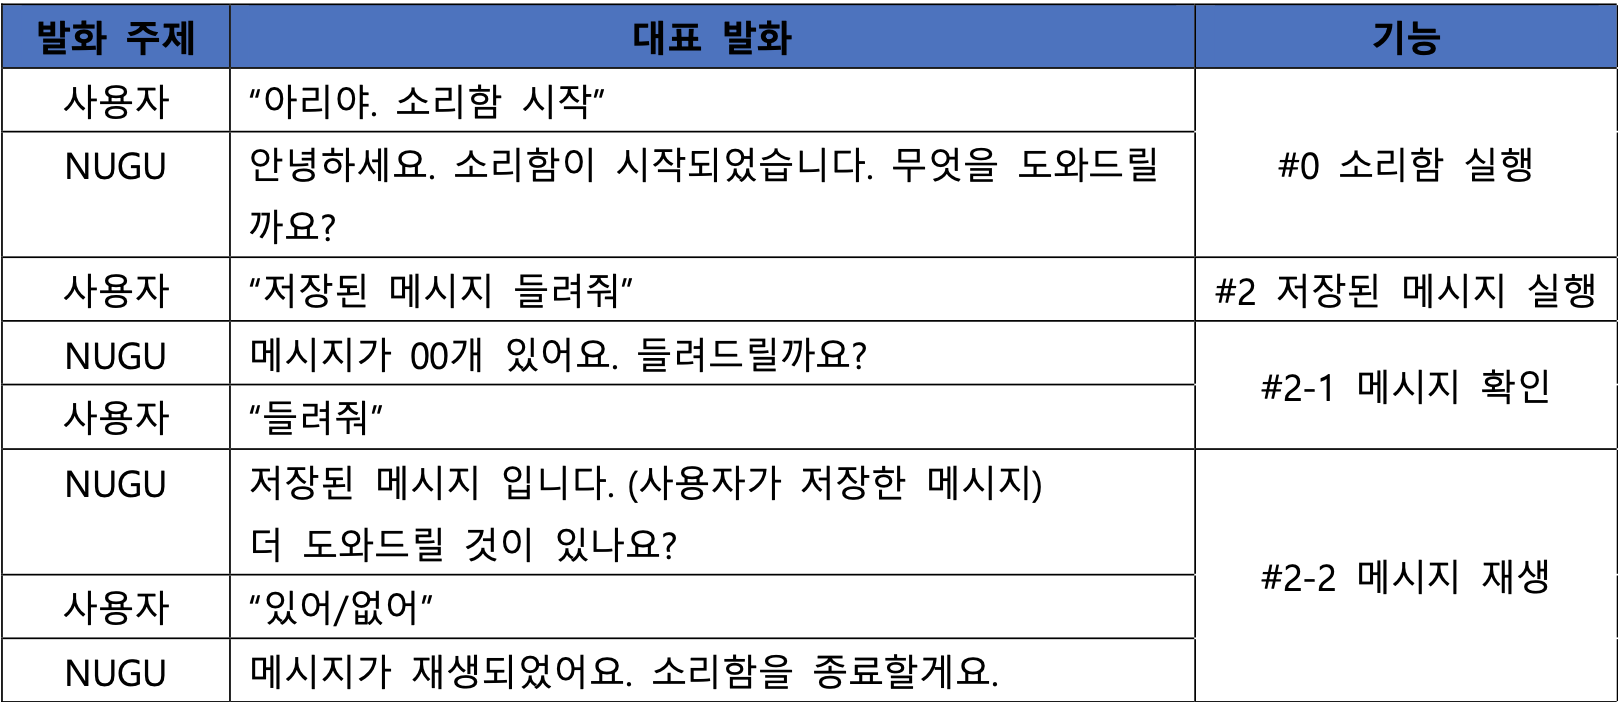
\includegraphics[width=9cm]{img/usecase 3.png}}
    \caption{User Case 3}
\end{figure}
- The user can wake up the speaker at any time to check the previously left message. After the user wakes up the speaker, he reveals his intention to "play the message." Then, the speaker understands the intention and takes 'SoundPlayAction'. The URL of the message left before in the storage is retrieved and played using the speaker's audio directive function.\\

\begin{thebibliography}{00}
\bibitem{b1} https://www.ncbi.nlm.nih.gov/pmc/articles/PMC3361774/.
\end{thebibliography}
\vspace{12pt}


\end{document}
